\def\year{2019}\relax
\documentclass[letterpaper]{article} % DO NOT CHANGE THIS
\usepackage{aaai19}  % DO NOT CHANGE THIS
\usepackage{times}  % DO NOT CHANGE THIS
\usepackage{helvet} % DO NOT CHANGE THIS
\usepackage{courier}  % DO NOT CHANGE THIS
\usepackage[hyphens]{url}  % DO NOT CHANGE THIS
\usepackage{graphicx} % DO NOT CHANGE THIS
\urlstyle{rm} % DO NOT CHANGE THIS
\def\UrlFont{\rm}  % DO NOT CHANGE THIS
\usepackage{graphicx}  % DO NOT CHANGE THIS
\frenchspacing  % DO NOT CHANGE THIS
\setlength{\pdfpagewidth}{8.5in}  % DO NOT CHANGE THIS
\setlength{\pdfpageheight}{11in}  % DO NOT CHANGE THIS
\nocopyright
\graphicspath{{images/}}
\usepackage{array}
\usepackage{amsmath}
\usepackage{caption}

\pdfinfo{
/Title (Text-to-Image Generation)
/Author (Mark Wesley Harris)
}

\setcounter{secnumdepth}{2} %May be changed to 1 or 2 if section numbers are 
%desired.

% The file aaai19.sty is the style file for AAAI Press 
% proceedings, working notes, and technical reports.
%
\setlength\titlebox{2.5in} % If your paper contains an overfull \vbox too high 
%warning at the beginning of the document, use this
% command to correct it. You may not alter the value below 2.5 in
\title{Text to Image Generation}
\author{Mark Wesley Harris\\
University of Colorado Colorado Springs\\
wharris2@uccs.edu
}
\begin{document}

\maketitle

\begin{abstract}
Before the late 20th century when capable technology was developed, humans had 
to rely on their own artistic talents in generating images.
Software programs, such as PhotoShop, were created to aid artists in generating 
images and editing photographs.
To this day, there are many computerized tools for artists to use, however it 
is clear that none of them are able to create images without external input. 
Some technologies, such as renderers used for animated movies and video games, 
break out of this trend, however they still consume vast amounts of resources 
and time in order to produce realistic outputs. Here we survey current 
technologies for text-to-image generation which may have the potential to aid 
in the rendering process, and with image generation as a whole.
\end{abstract}

\section{Introduction}
\label{sec:introduction}
Text to image generation is a widely studied problem in Computer Graphics. 
Since generating high quality images with a computer is impossible 
to perform analytically, researchers are now turning to machine learning to 
solve this and complex image processing problems.
Although the inception of deep image generation involved image-to-image 
translation, here we attempt to discern the best suited architecture for 
generating images given textual inputs. This is notably different from 
captioning images, which in general is easier but still very difficult. Our 
focus is on the robustness of existing machine learning algorithms and the 
fidelity of their results.

\section{Background}
Text-to-image generation is made possible through recent advancements in 
Computer Graphics and machine learning.
Two of the most popular concepts applied in the field are generative networks 
using adversarial learning, and attention mechanisms.
Most recently, researchers of text-to-image generation 
have combined both concepts, resulting in new architectures and better ways of 
processing data. In order to provide background for the contributions of each 
paper surveyed herein, an overview of generative adversarial learning and 
attention is provided below.

\subsection{Generative Adversarial Networks}
The Generative Adversarial Network (GAN)
was first proposed as a way to train a network to produce more realistic images
from random noise. The network is made up of two sub-architectures:
a generator, $G$, and a discriminator, $D$. The vanilla GAN model is 
essentially a random image generator, where the generated images share 
qualities of those in the training dataset. A generalization of the basic GAN 
architecture is shown in Figure \ref{fig:gan}.

\begin{figure}[htbp]
	\centerline{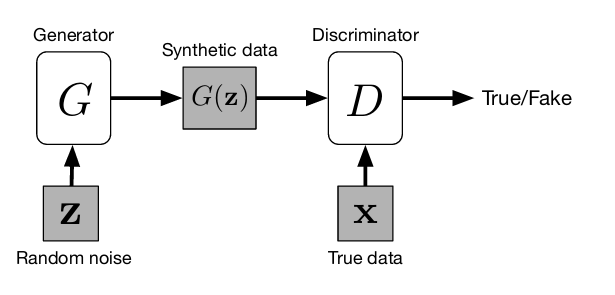
\includegraphics[width=7cm]{gan.png}}
	\caption{Basic Generative Adversarial Network architecture, with a 
		generator $G$
		and discriminator $D$
		\cite{cgan}.}
	\label{fig:gan}
\end{figure}

The generator is trained to progressively synthesize more realistic images,
while the discriminator is trained to recognize smaller differences between 
real and fake inputs \cite{cgan}. This relationship can be expressed in the 
format of a ``two-player min-max game'', which can be mathematically 
represented as in Equation \ref{eq:gan_basic}.
$p_{data}(\mathbf{x})$ represents the true data distribution,
and $p_{z}(\mathbf{z})$ represents the distribution of noise.

\begin{equation}
\label{eq:gan_basic}
\begin{split}
\text{min}_G\text{max}_DV(D,G) &=
E_{\mathbf{x}\sim p_{data}(\mathbf{x})}[\log D(\mathbf{x})] \\
&+ E_{\mathbf{z}\sim p_{z}(\mathbf{z})}[\log(1 - D(G(\mathbf{z})))]
\end{split}
\end{equation}

Many researchers found it difficult to train the basic GAN model to learn 
global  structures. Variation inference and other types of embedding was 
discovered to increase the quality of generated images \cite{varigan}. From 
these discoveries many variant architectures have been produced off of the 
original GAN model.The Deep Convolutional GAN (DCGAN)
was first proposed as a way to bridge the capabilities of unsupervised learning 
and supervised learning (such as Convolutional Neural Networks, called CNNs). 
The DCGAN has a similar structure to the original GAN model, but uses 
convolutional and convolutional-transpose layers in $D$ and $G$, respectively
\cite{unsupervised_learning}. Many frameworks also make use of an image 
enhancement architecture, such as the  Super Resolution GAN (SRGAN) proposed by 
\cite{srgan}. The SRGAN takes as input a low-resolution image with possible 
abnormalities, and outputs a larger, higher resolution image that is better 
quality. By combining these techniques and others, researchers created 
architectures such as the MSG-GAN, AttnGAN, and LeicaGAN.

\subsection{Attention Mechanisms}
Attention is a technique that references past data during each iteration of 
training. An attention function a mapping of a query and a
set of key-value pairs to an output \cite{attention_need}.
The mathematical expression of the attention function is shown in
Equation \ref{eq:attention}.
$d_k$ is the dimension of keys and queries, and
$Q,K,V$ are matrices of queries, keys, and values, respectively.
The function uses the dot product operator, so that the output is computed as
a linear combination of weights \cite{attention_need}.

\begin{equation}
\label{eq:attention}
\begin{split}
\text{Attention}(Q,K,V) = \text{softmax}(\frac{QK^T}{\sqrt{d_k}})V
\end{split}
\end{equation}

We can model the joint probability of a sequence,
$\mathbf{x}={x_1,x_2,\dots,x_n}$,
as the product of conditional
probability distributions parameterized by a network $\theta$
\cite{generative_transformers}.
The final expression is shown in Equation \ref{eq:attention_prob}.

\begin{equation}
\label{eq:attention_prob}
p(\mathbf{x}) = \prod_{i=1}^{n}p(x_i|x_1,\dots,x_{i-1};\theta)
\end{equation}

The first proposed attention mechanisms were accomplished by encoding with 
multiple Recurrent Neural Networks (RNNs). However, researchers found this 
strategy lacked efficiency. Transformers were first proposed
as a way to use attention mechanisms more efficiently.
The Transformer relies
``\dots entirely on self-attention to compute representations of its input and 
output
without using sequence-aligned RNNs or convolution''
\cite{attention_need}.
The encoder and decoder for the Transformer design
are shown in Figure \ref{fig:transformer}.
As demonstrated, an input is first encoded into the dimensional space
the Transformer works with, the network's weights are calculated,
and lastly the result is decoded back as the output of the model.
%The Transformer uses a series of attention functions to map
%between two sequences.
Transformers use a constant number of layers to model an arbitrary number of 
dependencies, which makes them useful for natural language processing and 
image generation \cite{generative_transformers}.

\begin{figure}[htbp]
\centerline{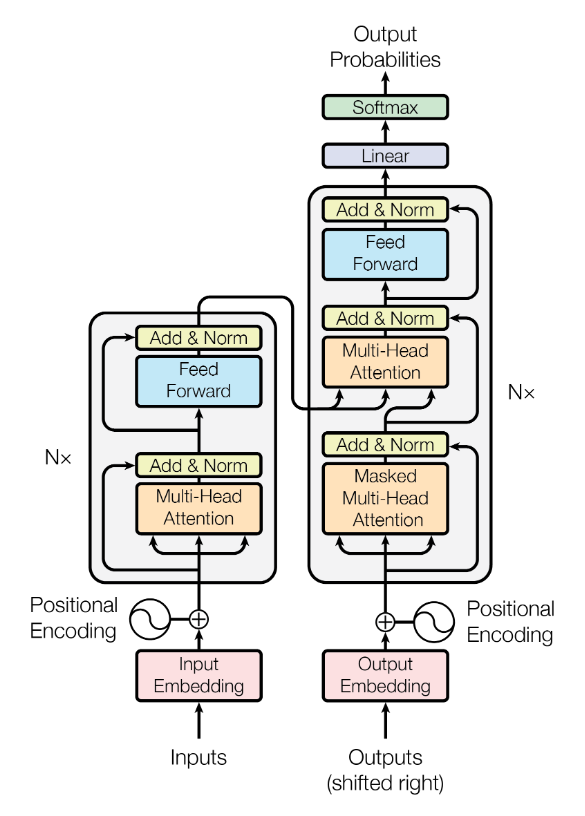
\includegraphics[width=7cm]{transformer.png}}
\caption{Transformer architecture showing Encoder and Decoder
\cite{attention_need}.}
\label{fig:transformer}
\end{figure}

%While the Transformer shows potential as a powerful machine learning technique,
%it is a recent concept and still has many inherent problems.
%One of the major problems with the architecture
%is that its required resources scales with $O(n^2)$
%for sequence length $n$. Researchers theorize that
%``\dots to improve computational performance for tasks involving very long 
%sequences,
%self-attention could be restricted to considering only a neighborhood of size 
%$r$''
%\cite{attention_need}.
%
%The Sparse Transformer architecture was developed as a means to shrink the
%computational resources for large sequences of data.
%Child et al. introduced sparse factorizations on the attention matrix
%in order to speed up processing.
%They approximated the dense attention
%operation by combining several cheaper attention operations.
%This new method resulted in a faster attention-based architecture
%that could be trained on longer sequences of data 
%\cite{generative_transformers}.
%
%\begin{figure}[htbp]
%\centerline{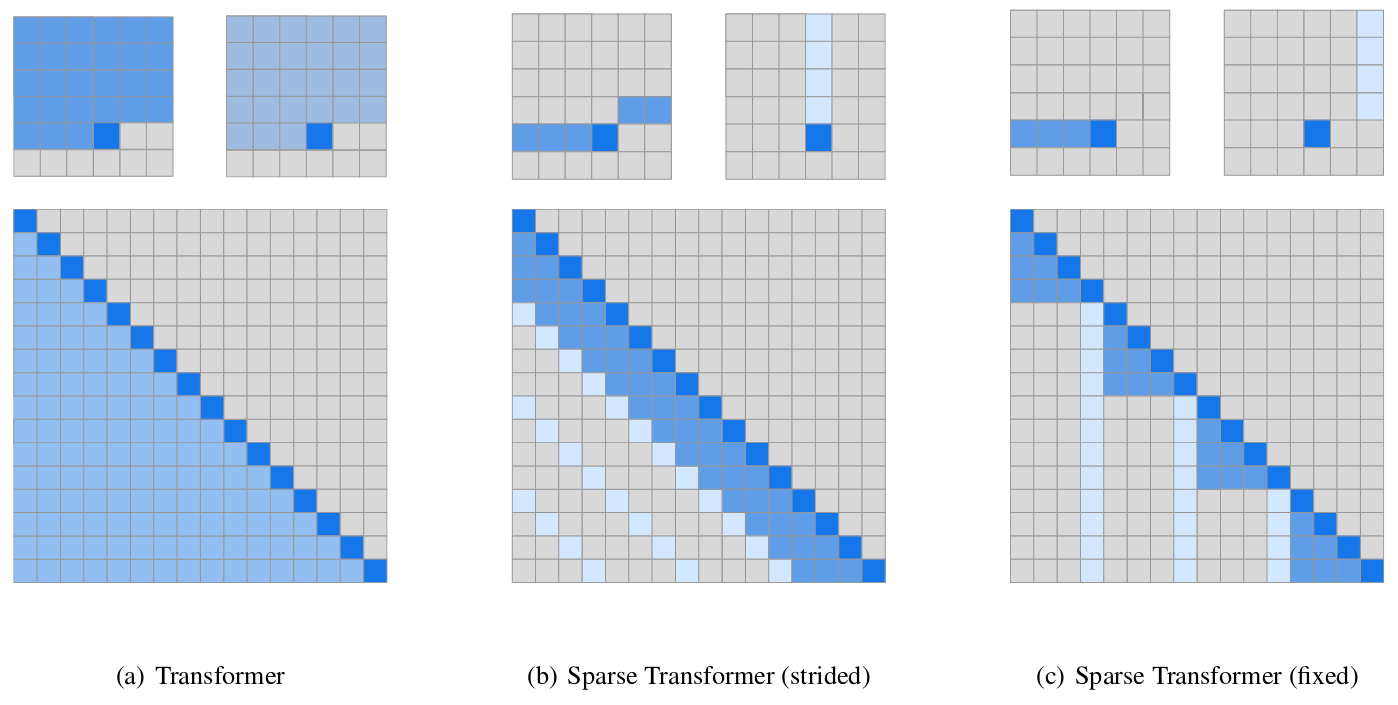
\includegraphics[width=7cm]{sparse_attention.png}}
%\caption{Optimizations of Attention
%\cite{generative_transformers}.}
%\label{fig:attention_optimization}
%\end{figure}
%
%Figure \ref{fig:attention_optimization} shows a visual representation of
%the two optimizations experimented with, strided and fixed.
%The Sparse Attention Transformer architecture reduces the resource cost to
%$O(n\sqrt[p]{n})$.
%The architecture is also simpler than other autoregressive models that perform
%similar functions, including upscaling and enhancement \cite{pixel_subscale}.

\section{Survey of Related Work}
While the topic of image generation as a whole is very broad, text-to-image 
generation using machine learning is a newer and lesser studied area. Starting 
as early as 2016 with Reed \textit{et al.}, GANs were applied to image 
generation given textual specifications. Research has continued to the present, 
where attention mechanisms are being applied as secondary inputs, such as with 
the AttnGAN \cite{attngan} and LeicaGAN \cite{leica} architectures. Here we 
cover some of the most prominent research, and explain its implications for the 
future of text-to-image synthesis.

%\subsection{Object-driven Text-to-Image Synthesis via Adversarial Training}
%\cite{objgan}

%\subsection{Text-Guided Attention Model for Image Captioning}
%\cite{attention_caption}

\subsection{Generative Adversarial Text to Image Synthesis, 2016}
The text-conditional convolutional GAN architecture was one of the first 
successful GAN architectures that experimented with text-to-image synthesis 
\cite{gan_text_to_image}. To train the generator, data was transmuted into a 
description embedding, denoted as the function $\varphi(t)$. This step is 
very similar to what is done in most text-processing machine learning models, 
such as the author's related work on deep representations in image 
classification \cite{deep_visual_descriptions}. Figure \ref{fig:cond_gan} shows 
the developed GAN architecture, which is similar to 
the DCGAN discussed previously. Notably, this is the simplest and earliest 
architecture of those proposed for this problem. Reed \textit{et al.}
also developed a way to experiment with the matching-aware
discriminator (GAN-CLS) and manifold interpolation (GAN-INT) mechanisms. They 
found through testing that a combination of these optimizations gave better 
qualitative results than their base DCGAN model. This work demonstrates how 
GANs can be stabilized with improved ways of extracting important information 
from unrelated data, which indeed is necessary for the difficult task of 
text-to-image generation.

\begin{figure}[htbp]
\centerline{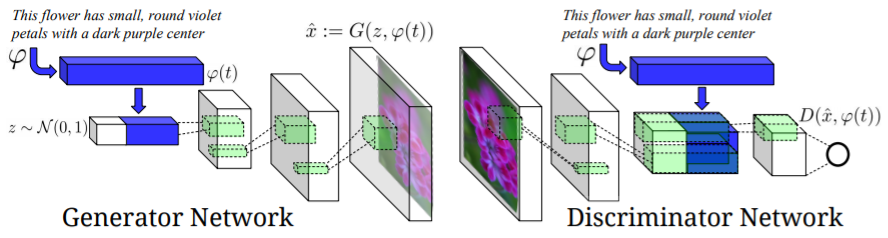
\includegraphics[width=8cm]{cond_gan.png}}
\caption{Text-conditional convolutional GAN architecture, with textual 
description embedding \cite{gan_text_to_image}.}
\label{fig:cond_gan}
\end{figure}

%\subsection{Learning Deep Representations of Fine-Grained Visual 
%Descriptions, 2016}
%\cite{deep_visual_descriptions}

%\subsection{StackGAN++: Realistic Image Synthesis
%with Stacked Generative Adversarial Networks, 2017}
%\cite{stackgan++} also found problems with GAN stability.

\subsection{AttnGAN: Fine-Grained Text to Image Generation
with Attentional Generative Adversarial Networks, 2017}
Text-to-image generation was notably improved by Microsoft Research 
with the advent of the Attentional GAN (AttnGAN) model \cite{attngan}.
The AttnGAN architecture (shown in Figure \ref{fig:attngan}) combines the 
inherent inference obtained by the generator and discriminator within the GAN 
framework, with the improvements in dependency correlation and stability gained 
from attention. Instead of encoding the entire sentence as a single input 
vector (e.g. ``this bird has wings that are blue and a red belly``), each word 
in the sentence is allowed an opportunity to claim regional importance in the 
output image. This ability provides better recognition of conditional 
sub-regions, which improves overall semantic relevance of the output image.  
AttnGAN was also based on the work of the StackGAN++ architecture, which found 
a multi-stage approach was necessary for stabilizing sensitivities in training 
GAN models \cite{stackgan++}. Figure \ref{fig:attngan_sample} shows a sample 
input and corresponding output for the AttnGAN model as well as the results of 
attention, demonstrating the semantic relevance of the output image.

\begin{figure}[htbp]
	\centerline{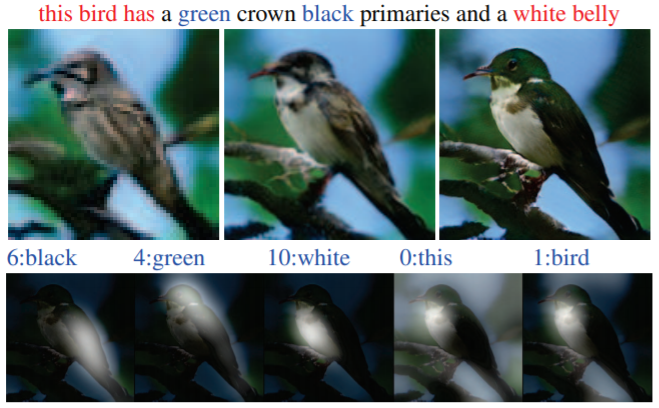
\includegraphics[width=7cm]{attngan_sample.png}}
	\caption{Intermediate and final outputs for AttnGAN (top) and the trained 
	attention map (bottom)
		\cite{attngan}.}
	\label{fig:attngan_sample}
\end{figure}

%\subsection{MirrorGAN: Learning Text-to-image Generation by Redescription}
%\cite{mirrorgan}

\subsection{MSG-GAN: Multi-Scale Gradients for Generative Adversarial
Networks, 2019}
The Multi-Scale Gradient GAN (MSG-GAN) was the first GAN to generate images 
with very high resolutions (up to 1024 x 1024 pixels).
Researchers have found it difficult to produce high-resolution images with GANs
``
%This problem is more severe when training GANs to generate
%high-resolution (e.g., 256x256) images
\dots because the chance is
very low for the image distribution and the model distribution
to share supports in a high-dimensional space
'' \cite{stackgan++}.
The MSG-GAN, however, provides mechanisms used by the discriminator to 
reference all resolutions of images generated, which double in size starting as 
small as 4 x 4. By referencing the outputs of all intermediate layers, the 
MSG-GAN acquires more stability during training, and thus produces better 
outputs for all generated resolutions
%``
%MSG-GAN allows
%the discriminator to look at not only the final output (highest resolution) of 
%the generator, but also at the outputs of
%the intermediate layers 
%''
\cite{msggan}. Figure \ref{fig:msggan} shows results of the MSG-GAN generating 
very small (left) and very high (right) resolutions for a given input.
Their approach will undoubtedly revolutionize how we generate images in the 
future, especially for high-resolution outputs such as rendered frames.

\begin{figure}[htbp]
	\centerline{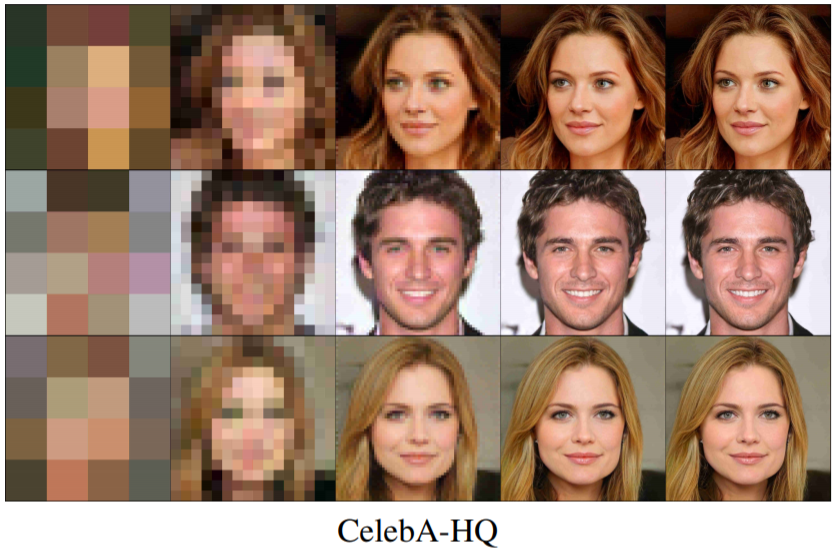
\includegraphics[width=7cm]{msggan.png}}
	\caption{MSG-GAN results for increasing resolutions
		\cite{msggan}.}
	\label{fig:msggan}
\end{figure}

\subsection{Learn, Imagine and Create: Text-to-Image Generation from Prior 
Knowledge, 2019}
A new architecture was created from the advancements of AttnGAN, called LEarn, 
Imagine and CreAte GAN (LeicaGAN) \cite{leica}. Similar to other 
attention-based GANs, the LeicaGAN architecture is comprised of a 
text-embedding phase, followed by coarse-to-fine image generators. The main 
difference in the LeicaGAN is their use of textual-visual co-embedding (TVE) 
and multiple priors aggregation (MPA) to further extract semantic meaning from 
their inputs. The authors argue that their architecture more closely models how 
the human brain analyzes textual data, and therefore will have better results 
in identifying the relationships between an image and its textual description.

\begin{figure}[htbp]
	\centerline{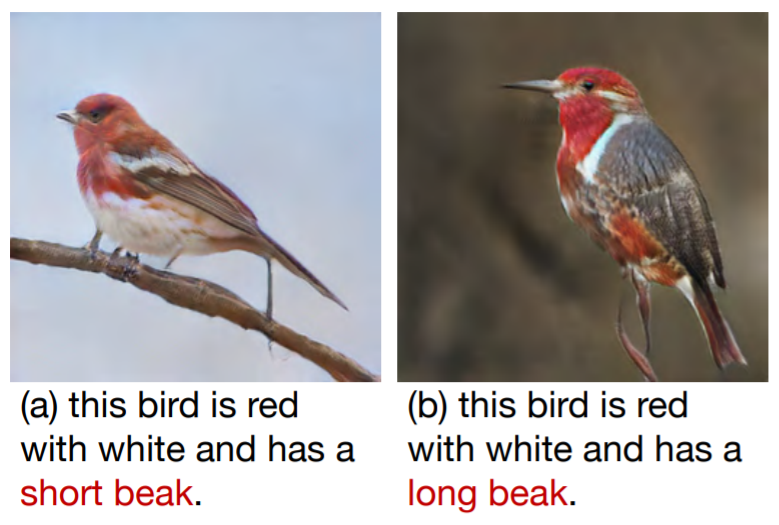
\includegraphics[width=7cm]{leicagan_sample.png}}
	\caption{Image outputs of LeicaGAN for similar input sentences
		\cite{leica}.}
	\label{fig:leica_sample}
\end{figure}

Figure \ref{fig:leica_sample} demonstrates how images may differ from changing 
one attribute only. A by-product of this change is that the setting and pose 
are completely different. Further analysis is needed to determine how much of 
this can be controlled analytically. Figure \ref{fig:leicagan} shows the 
results of LeicaGAN on the CUB bird and Oxford-102 flower datasets, as well as 
results of AttnGAN for comparison. Their analysis shows that LeicaGAN is 
objectively better than previous state-of-the-art methods for text-to-image 
generation.

%\section{Evaluation Criteria}
%A major criticism of GANs and other generative models is the
%``lack of a robust and consistent evaluation method\dots''
%\cite{gmm}.
%As opposed to other machine learning models, GANs do not optimize any kind of 
%objective function,
%and operate instead on a learned latent space
%which cannot be analyzed analytically.
%Thus, in order to evaluate the implemented models,
%we must find a way to numerically compare the generated images to their 
%respective targets.
%
%Researchers have defined many different means of comparing two images.
%Some of this research is focused on image context, such as if two images 
%contain the same
%person or setting.
%This type of analysis would not benefit our project,
%since the image needs to be exact --
%simply containing similar features is not enough.
%Thus, we turned to the measurements of
%Mean Squared Error (MSE) and Peak Signal-To-Noise Ratio (PSNR),
%as both metrics are commonly used to evaluate super resolution algorithms
%\cite{super_resolution}.

%``
%Inception Score and R-precision are regarded as effective and are commonlyused 
%for evaluating the diversity of the generated images \dots it was observed 
%that 
%a
%text-to-image model could get a fairly high performance even when the model 
%actually generated
%visually-low quality images
%''
%\cite{leica}.

%\section{Work Completed}
%\begin{figure}[htbp]
%\centerline{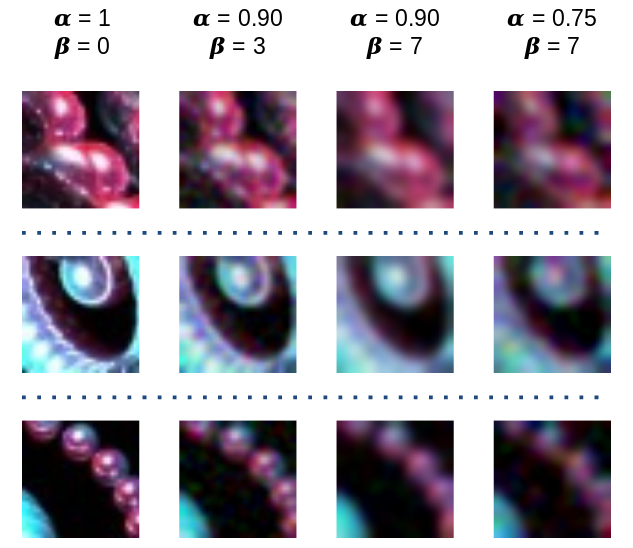
\includegraphics[width=8cm]{altered_data.png}}
%\caption{.}
%\label{fig:altered}
%\end{figure}

\section{Conclusion}
\label{sec:conclusion}
Since the dawn of humanity, manually creating images through drawing, 
painting, or rendering has been the only available method for image generation. 
However the recent application of complex artificial neural networks
has broken through the creative glass ceiling, and opened the door to new image 
generation prospects. With the advent of Generative Adversarial Networks, we 
now have models capable of generating images. Since many researchers found that 
conditional GANs can easily become unstable and sometimes generate 
undesired results, they are now utilizing the concept of 
attention to synthesize higher-quality images with more semantic relevance. 
The AttnGAN and LeicaGAN architectures are both excellent examples of mature 
text-to-image generation models. We look forward to seeing the application of 
these models to context-aware image generation, as well as other difficult 
problems in the field of Computer Graphics and Computer Vision.

\begin{figure*}[htbp]
	\centerline{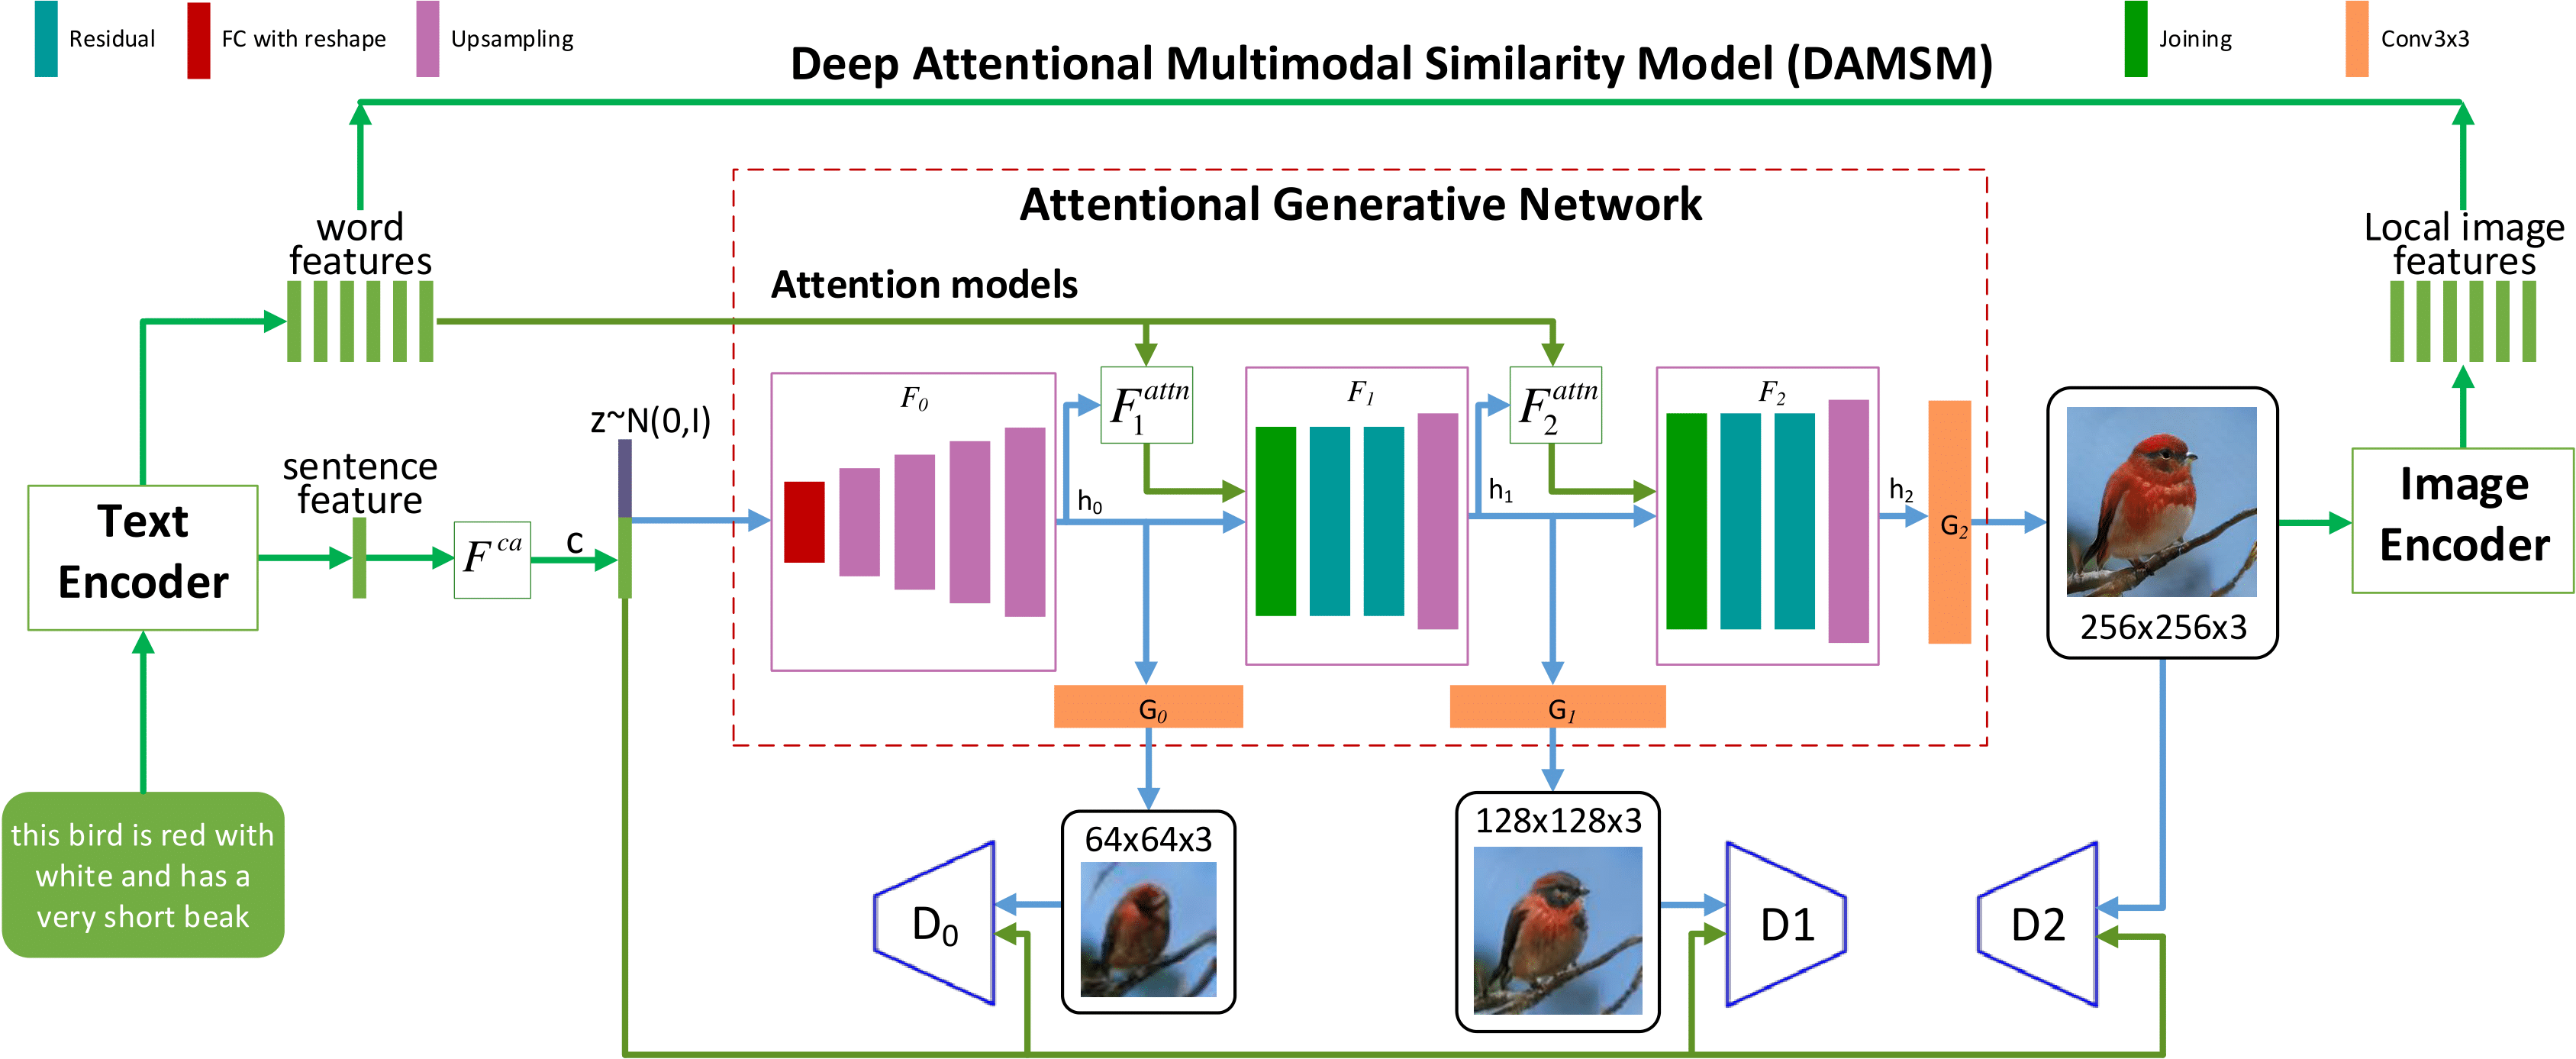
\includegraphics[width=\linewidth]{attngan.png}}
	\caption{AttnGAN architecture, showing separate generators and introduction 
		of Attention mechanisms.}
	\label{fig:attngan}
\end{figure*}

\begin{figure*}[htbp]
	\centerline{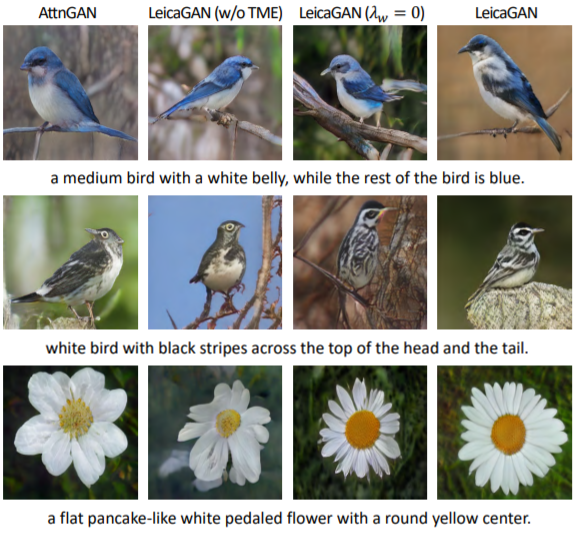
\includegraphics[width=\linewidth]{leicagan.png}}
	\caption{LeicaGAN results with varied hyperparameters, compared to results 
		of AttnGAN
		\cite{leica}.}
	\label{fig:leicagan}
\end{figure*}

\bibliography{midterm}
\bibliographystyle{aaai}

\end{document}
